\section{Pregunta N$^{\circ}$7\qquad Andre Gilmer Santos Felix}

\begin{frame}
	\begin{enumerate}\setcounter{enumi}{6}
		\item

		      Encuentre el interpolante de Lagrange
		      \begin{math}
			      p_{3}\left(t\right)=
			      \sum\limits_{k=0}^{3}
			      x_{k}
			      \ell_{k}\left(t\right)
		      \end{math}
		      para el conjunto de datos
		      \begin{math}
			      \left\{
			      \left(0,1\right),
			      \left(\dfrac{1}{2},2\right),
			      \left(1,\dfrac{3}{2}\right),
			      \left(2,-1\right)
			      \right\}
		      \end{math}.
		      Encuentre $p_{2,k}$ en
		      \begin{math}
			      p_{3}\left(t\right)=
			      \sum\limits_{k=0}^{3}
			      p_{3,k}t^{k}
		      \end{math}.
	\end{enumerate}

	\begin{solution}
		Determinamos las funciones base de Lagrange
		\begin{math}
			{\left\{\ell_{k}\right\}}^{3}_{k=0}\subset\mathbb{P}_{3}
		\end{math}.

		\begin{align*}
			\ell_{0}\left(t\right) & =
			\prod\limits_{\substack{j=0               \\j\neq 0}}^{3}
			\dfrac{t-t_{j}}{t_{0}-t_{j}}=
			\dfrac{
				\left(t-t_{1}\right)
				\left(t-t_{2}\right)
				\left(t-t_{3}\right)
			}{
				\left(t_{0}-t_{1}\right)
				\left(t_{0}-t_{2}\right)
				\left(t_{0}-t_{3}\right)
			}=
			\dfrac{
				\left(t-\dfrac{1}{2}\right)
				\left(t-1\right)\left(t-2\right)
			}{
				\left(0-\dfrac{1}{2}\right)
				\left(0-1\right)
				\left(0-2\right)
			}=
			-t^{3}+\dfrac{7}{2}t^{2}-\dfrac{7}{2}t+1. \\
			\ell_{1}\left(t\right) & =
			\prod\limits_{\substack{j=0               \\j\neq 1}}^{3}
			\dfrac{t-t_{j}}{t_{1}-t_{j}}=
			\dfrac{
				\left(t-t_{0}\right)
				\left(t-t_{2}\right)
				\left(t-t_{3}\right)
			}{
				\left(t_{1}-t_{0}\right)
				\left(t_{1}-t_{2}\right)
				\left(t_{1}-t_{3}\right)
			}=
			\dfrac{
				\left(t-0\right)
				\left(t-1\right)
				\left(t-2\right)
			}{
				\left(\dfrac{1}{2}-0\right)
				\left(\dfrac{1}{2}-1\right)
				\left(\dfrac{1}{2}-2\right)
			}=
			\dfrac{8}{3}t^{3}-8t^{2}+\dfrac{16}{3}t.  \\
			\ell_{2}\left(t\right) & =
			\prod\limits_{\substack{j=0               \\j\neq 2}}^{3}
			\dfrac{t-t_{j}}{t_{2}-t_{j}}=
			\dfrac{
				\left(t-t_{0}\right)
				\left(t-t_{1}\right)
				\left(t-t_{3}\right)
			}{
				\left(t_{2}-t_{0}\right)
				\left(t_{2}-t_{1}\right)
				\left(t_{2}-t_{3}\right)
			}=
			\dfrac{
				\left(t-0\right)
				\left(t-\dfrac{1}{2}\right)
				\left(t-2\right)
			}{
				\left(1-0\right)
				\left(1-\dfrac{1}{2}\right)
				\left(1-2\right)
			}=
			-2t^{3}+5t^{2}-2t.                        \\
			\ell_{3}\left(t\right) & =
			\prod\limits_{\substack{j=0               \\j\neq 3}}^{3}
			\dfrac{t-t_{j}}{t_{3}-t_{j}}=
			\dfrac{
				\left(t-t_{0}\right)
				\left(t-t_{1}\right)
				\left(t-t_{2}\right)
			}{
				\left(t_{3}-t_{0}\right)
				\left(t_{3}-t_{1}\right)
				\left(t_{3}-t_{2}\right)
			}=
			\dfrac{
				\left(t-0\right)
				\left(t-\dfrac{1}{2}\right)
				\left(t-1\right)
			}{
				\left(2-0\right)
				\left(2-\dfrac{1}{2}\right)
				\left(2-1\right)
			}=
			\dfrac{1}{3}t^{3}-\dfrac{1}{2}t^{2}+\dfrac{1}{6}t.
		\end{align*}
	\end{solution}
\end{frame}

\begin{frame}
	\begin{solution}
		Entonces, el polinomio interpolador de Lagrange es
		\begin{align*}
			p_{3}\left(t\right) & =
			\sum\limits_{k=0}^{3}
			x_{k}
			\ell_{k}\left(t\right)=
			\alert{x_{0}}
			\ell_{0}\left(t\right)+
			\alert{x_{1}}
			\ell_{1}\left(t\right)+
			\alert{x_{2}}
			\ell_{2}\left(t\right)+
			\alert{x_{3}}
			\ell_{3}\left(t\right)=
			\left(
			\alert{1}
			\right)
			\ell_{0}
			\left(t\right)+
			\left(
			\alert{2}
			\right)
			\ell_{1}\left(t\right)+
			\left(
			\alert{\dfrac{3}{2}}
			\right)
			\ell_{2}\left(t\right)+
			\left(
			\alert{-1}
			\right)
			\ell_{3}\left(t\right). \\
			                    & =
			\left(
			\alert{
				-t^{3}+\dfrac{7}{2}t^{2}-\dfrac{7}{2}t+1
			}
			\right)+
			2
			\left(
			\alert{
				\dfrac{8}{3}t^{3}-8t^{2}+\dfrac{16}{3}t
			}
			\right)-
			\dfrac{3}{2}
			\left(
			\alert{
				-2t^{3}+5t^{2}-2t
			}
			\right)-
			\left(
			\alert{
				\dfrac{1}{3}t^{3}-\dfrac{1}{2}t^{2}+\dfrac{1}{6}t
			}
			\right)                 \\
			                    & =
			t^{3}-\dfrac{9}{2}t^{2}+4t+1.
		\end{align*}
	\end{solution}
\end{frame}

\begin{frame}
	\begin{solution}
		\begin{figure}[ht!]
			\centering
			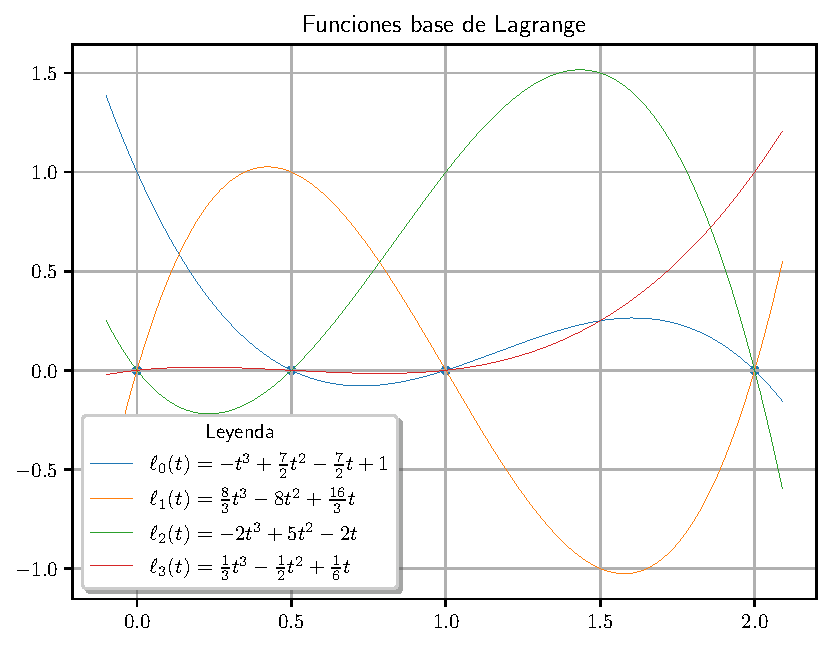
\includegraphics[width=.72\paperwidth]{p7_lagrange}
		\end{figure}
	\end{solution}
\end{frame}


\begin{frame}
	\begin{solution}
		\begin{figure}[ht!]
			\centering
			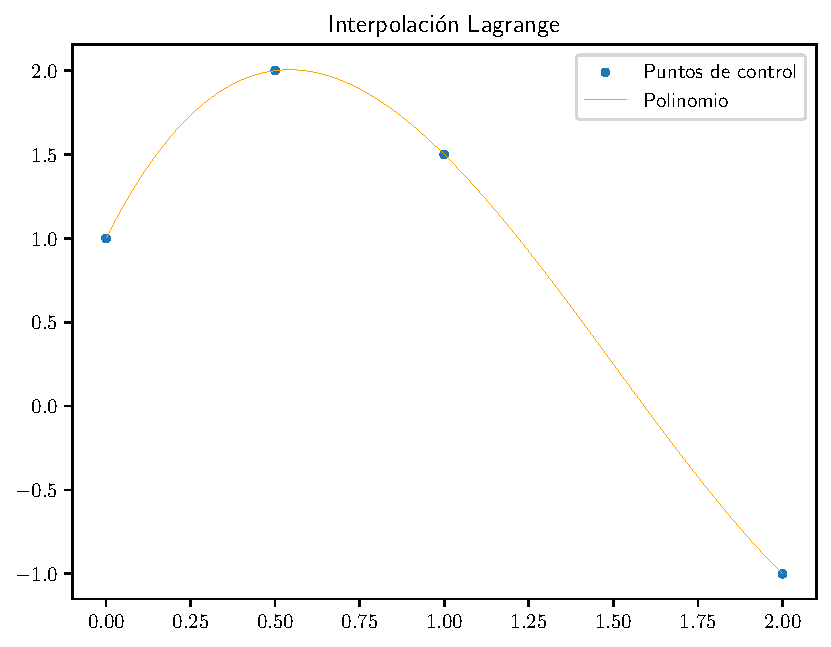
\includegraphics[width=.72\paperwidth]{p7}
		\end{figure}
	\end{solution}
\end{frame}